%%%%%%%%%%%%%%%%%%%%%%%%%%%%%%%%%%%%%%%%%%%%%%%%%%%%%%%%%%%%%%%%%%%%%%
% Overleaf (WriteLaTeX) Example: Molecular Chemistry Presentation
%
% Source: http://www.overleaf.com
%
% In these slides we show how Overleaf can be used with standard
% chemistry packages to easily create professional presentations.
%
% Feel free to distribute this example, but please keep the referral
% to overleaf.com
%
%%%%%%%%%%%%%%%%%%%%%%%%%%%%%%%%%%%%%%%%%%%%%%%%%%%%%%%%%%%%%%%%%%%%%%
% How to use Overleaf:
%
% You edit the source code here on the left, and the preview on the
% right shows you the result within a few seconds.
%
% Bookmark this page and share the URL with your co-authors. They can
% edit at the same time!
%
% You can upload figures, bibliographies, custom classes and
% styles using the files menu.
%
% If you're new to LaTeX, the wikibook is a great place to start:
% http://en.wikibooks.org/wiki/LaTeX
%
%%%%%%%%%%%%%%%%%%%%%%%%%%%%%%%%%%%%%%%%%%%%%%%%%%%%%%%%%%%%%%%%%%%%%%

\documentclass{beamer}

% For more themes, color themes and font themes, see:
% http://deic.uab.es/~iblanes/beamer_gallery/index_by_theme.html
%
\mode<presentation>
{
  \usetheme{Madrid}       % or try default, Darmstadt, Warsaw, ...
  \usecolortheme{default} % or try albatross, beaver, crane, ...
  \usefonttheme{serif}    % or try default, structurebold, ...
  \setbeamertemplate{navigation symbols}{}
  \setbeamertemplate{caption}[numbered]
}

\usepackage[english]{babel}
\usepackage[utf8x]{inputenc}
\usepackage{chemfig}
\usepackage[version=3]{mhchem}

% On Overleaf, these lines give you sharper preview images.
% You might want to `comment them out before you export, though.
\usepackage{pgfpages}
\pgfpagesuselayout{resize to}[%
  physical paper width=8in, physical paper height=6in]


\title[Malliavin Calculus and MC]{Applications of Malliavin Calculus to Monte-Carlo Methods in Finance}
\author{E. Fourni$\acute{e}$, J-M Lasry, J. Lebuchoux, P-L Lions}
%\institute{www.overleaf.com}
\date{\today}

\begin{document}


% Page 1, title author and date
\begin{frame}
  \titlepage
\end{frame}


% Page 2, outline of the paper/slides
\begin{frame}{Outline}
  \tableofcontents
\end{frame}

%%%%%%%%%%%%%%%%%%%%%%%%%%%%%%%%%%%%%%%%%%%%%%%%%%%%%%%%%%%%%%
\section{Introduction}


% Page 3, motivation of the paper
\begin{frame}{Motivation}
In finance, the demand of hedging financial instruments, especially (exotic) options is based on the calculation of {\emph \bf Greeks}
\begin{itemize}
  \item explicit formula (very simple examples, e.g. European Call);
  \item Monte Carlo Simulation the finite difference approximation of the differentials
  \begin{itemize}
      \item{perform very poorly when pay-off function is not smooth enough}
      \item{hard to handle complex pay-off function case with accuracy}
      \item{inadequacy for the treatment of American-type options (part II)}
    \end{itemize}
\end{itemize}
\end{frame}


% Page 4, some mathematical notations
\begin{frame}{Some Mathematical Notations...}
  The underlying assets are assumed to be given by $\{X(t); 0\leq t \leq T\}$, whose dynamic are described by stochastic differential equation
  $$
  dX(t) = b(X(t))dt + \sigma(X(t)) dW(t)
  $$
  where $\{W(t), 0\leq t \leq T\}$ is a Brownian motion with values in $\mathbb{R}^n$.

  \bigskip
  \bigskip

  Given $0 \leq t_1 \leq \ldots \leq t_m = T$, we consider the function
  $$
  u(x) = \mathbb{E}[\phi(X(t_1),\ldots,X(t_m)) | X(0) = x]
  $$
  where $u(x)$ describes the prices of a contingent claim defined by the pay-off function $\phi$ involving the times $(t_1,\ldots,t_m)$.
\end{frame}


% Page 5, Contributions of the paper
\begin{frame}{Main findings and contributions of this paper}
  In this paper, using Malliavin calculus we will show that all the differentials
of interest can be expressed as
  $$
  \mathbb{E}[\pi \phi(X(t_1),\ldots,X(t_m)) | X(0) = x]
  $$
  where the weight $\pi$ does not depend on the pay-off function $\phi$.
\end{frame}


% Page 6, some simplified theories
\begin{frame}{Some simplified theoretical aspects}
  The asset prices can be written
  $$
  price = \mathbb{E}_{Q_0}[\textrm{pay-offs}]
  $$
  where $\mathbb{E}_{Q_0}$ is the expected value under the risk neutral probability $Q_0$. The marginal changes of $Q$ will lead to new prices according to
  \begin{eqnarray*}
  variation~of~prices &=& new~prices - old~prices \\
  					  &=& \mathbb{E}_{Q}[\textrm{pay-offs}] -\mathbb{E}_{Q_0}[\textrm{pay-offs}] \\
                      &=& \mathbb{E}_{Q_0}[\textrm{pay-offs} \times \pi]
  \end{eqnarray*}
  where
  $$
  \pi = \frac{dQ-dQ_0}{dQ_0}
  $$
\end{frame}


% Page 7, some simplified theories, con't
\begin{frame}{Some simplified theoretical aspects, con't}
  Suppose that the probability $Q$ lies within a parametrized family $(Q_\lambda)$. $\lambda = (\lambda_1,\ldots,\lambda_n)$. Then the marginal moves of the market can be assessed
through the derivatives
  $$
  \frac{\partial}{\partial \lambda_i} (price) = \mathbb{E}_{Q_0}[\textrm{pay-offs} \times \pi_i]
  $$
  where $G = \frac{dQ}{dQ_0}$ and $\pi_i=\frac{\partial G}{\partial \lambda_i}$, i.e. $\pi_i$ is the logarithmic derivative of $Q$ at $Q_0$ in the $\lambda_i$ direction.
\end{frame}

%%%%%%%%%%%%%%%%%%%%%%%%%%%%%%%%%%%%%%%%%%%%%%%%%%%%%%%%%%%%%%

\section{Malliavin Calculus in Finance}

% Page 8, notations for malliavin calculus
\begin{frame}{Notations}
Let $\{W(t),0\leq t \leq T\}$ be a n-dimensional Brownian motion defined on a complete probability space $(\omega, \mathcal{F}, P)$. Let $\mathcal{L}$ be the set of r.v. $F$ of the form
$$
F = f\left( \int_0^\infty h_1(t)dW(t),\ldots, \int_0^\infty h_n(t)dW(t) \right), \quad f\in \mathcal{P}(\mathbb{R}^n)
$$
where $\mathcal{P}(\mathbb{R}^n)$ denotes the set of infinitely differentiable and rapidly decreasing function on $\mathbb{R}^n$ and $h_1,\ldots,h_n\in L^2(\omega \times \mathbb{R}_+)$. The Malliavin derivative $DF$ of $F$ is defined as the process $\{D_t F, t\geq 0\}$ of $L^2(\omega \times \mathbb{R}_+)$ with values in $L^2(\mathbb{R}_+)$ which we denote by $H$
$$
D_t F = \sum_{i=1}^{n} \frac{\partial}{\partial x_i} \left( \int_0^\infty h_1(t)dW(t),\ldots, \int_0^\infty h_n(t)dW(t) \right)h_t(t), \quad t\geq 0~a.s.
$$
\end{frame}


% Page 9, properties of malliavin calculus
\begin{frame}{Properties of Malliavin Calculus}
\textbf{Property 1}. Let $\phi: \mathbb{R}^n \rightarrow \mathbb{R}$ be a continuously differentiable function with partial derivatives and $F=(F_1,\ldots,F_n)$ a random vector whose components belong to $\mathbb{D}^{1,2}$. Then $\phi(F)\in \mathbb{D}^{1,2}$ and
$$
D_t \phi(F) = \sum_{i=1}^{n} \frac{\partial \phi}{\partial x_i} (F) D_t F_i, \qquad t\geq 0~a.s.
$$
\end{frame}


% Page 10, properties of malliavin calculus, con't
\begin{frame}{Properties of Malliavin Calculus,con't}
\textbf{Property 2}. Let $\{Y(t), t\geq 0\}$ be the associated first variation process of $X(t)$ and
$$
dY(t) = b'(X(t))Y(t)dt + \sum_{i=1}^n \sigma_i'(X(t))Y(t) dW^i(t), \quad Y(0) = I_n
$$
where $I_n$ is the identity matrix of $\mathbb{R}^n$, primes denote derivatives and $\sigma_i$ is the
$i$-th column vector of $\sigma$. Then the process $\{X(t), t\geq 0\}$ belongs to $\mathbb{D}^{1,2}$ and its Malliavin derivative is given by
$$
D_s X(t) = Y(t)Y^{-1}(s)\sigma(X(s)) 1_{\{s\leq t\}}, \quad s\geq 0~a.s.
$$
Hence, if $\psi\in C^1_b(\mathbb{R}^n)$ then we have
\begin{eqnarray*}
D_s \psi(X_T) &=& \nabla \psi(X_T)Y(T)Y^{-1}(s)\sigma(X(s)) 1_{\{s\leq T\}}, \quad s\geq 0~a.s. \\
D_s \int_0^\infty \psi(X_t) dt &=& \int_s^T \nabla \psi(X_T)Y(T)Y^{-1}(s)\sigma(X(s)) dt \quad a.s. \\
\end{eqnarray*}
\end{frame}

% Page 11, properties of malliavin calculus, con't
\begin{frame}{Properties of Malliavin Calculus,con't}
\textbf{Property 3}. Let $u$ be a stochastic process. Then $u\in Dom(\delta)$ if for any $\phi\in \mathbb{D}^{1,2}$, we have
$$
\mathbb{E}(<D\phi,u>_H) = \mathbb{E} \left( \int_0^\infty D_t \phi u(t) dt \right) \leq C(u) ||\phi||_{1,2}
$$
if $u\in Dom(\delta)$, we define $\delta(u)$ by
$$
\mathbb{E}(\phi\delta(u)) = \mathbb{E}(<D\phi,u>_H) \quad for~any~\phi \in \mathbb{D}^{1,2}
$$
\end{frame}

% Page 12, properties of malliavin calculus, con't
\begin{frame}{Properties of Malliavin Calculus,con't}
\textbf{Property 4}. Let $u$ be an adapted stochastic process in $L^2(\omega \times \mathbb{R}_+)$. Then we have
$$
\delta(u) = \int_0^\infty [u(t)]^* dW(t)
$$

\textbf{Property 5}. Let $F$ be an $\mathcal{F}_T-$adapted random variable which belongs to $\mathbb{D}^{1,2}$ then for any $u$ in $dom(\delta)$ we have
$$
\delta(Fu) = F\delta(u) - \int_0^T D_t F u(t) dt
$$

\textbf{Property 6}. Let $F$ be an a random variable which belongs to $\mathbb{D}^{1,2}$. Then we have
$$
F = \mathbb{F} + \int_0^T \mathbb{E}(D_tF|\mathcal{F}_t) dW(t)
$$
\end{frame}


%%%%%%%%%%%%%%%%%%%%%%%%%%%%%%%%%%%%%%%%%%%%%%%%%%%%%%%%%%%%%%

\section{Greeks Calculation with Malliavin}

% Page 13, assumption on variations
\begin{frame}{Greeks calculation: assumption}
We denote by $\{Y(t), 0 \leq t \leq T\}$ the first variation process associated to $\{X(t), 0 \leq t \leq T\}$ defined by the stochastic differential equation
\begin{eqnarray*}
Y(0)  &=& I_n \\
dY(t) &=& b'(X(t))Y(t)dt + \sum_{i=1}^n \sigma_i'(X(t)) Y(t) dW_i(t)
\end{eqnarray*}

\textbf{Assumption 3.1} The diffusion matrix  satisfies the uniform ellipticity condition
$$
\exists \epsilon >0, \xi^* \sigma^*(x)\sigma(x)\xi \geq \epsilon |\xi|^2 \quad for~any~\xi,x \in \mathbb{R}^n
$$
\end{frame}


% Page 14, Variation in the drift coefficient
\begin{frame}{Variations in the drift coefficient and initial condition}
\textbf{Property 3.1}. The function $\epsilon \mapsto u^\epsilon(x)$ is differentiable in $\epsilon = 0$, for any $x\in \mathbb{R}^n$, and we have
$$
\left. \frac{\partial}{\partial \epsilon} u^\epsilon(x) \right|_{\epsilon=0} = \mathbb{E}\left[ \left. \phi(X(.))\int_0^T <\sigma^{-1}\gamma(X(t)),dW(t)> \right| X(0) = x \right]
$$

\textbf{Property 3.2}. Under Assumption 3.1, for any $x\in \mathbb{R}^n$ and for any $a\in\Gamma_m$, we
have
$$
\nabla u(x) = \mathbb{E}^x \left[ \phi(X(t_1),\ldots,X(t_m))\int_0^T a(t)[\sigma^{-1}(X(t))(Y(t))]^*dW(t)  \right]
$$
\end{frame}

% Page 15, Variation in the diffusion coefficient
\begin{frame}{Variations in the diffusion coefficient}
\textbf{Assumption 3.2}. The diffusion matrix  $\sigma+\epsilon\tilde{\sigma}$ satisfies the uniform ellipticity condition for any $\epsilon$
$$
\exists \eta >0, \xi^* (\sigma+\epsilon\tilde{\sigma})^*(x)(\sigma+\epsilon\tilde{\sigma})(x)\xi \geq \eta |\xi|^2 \quad for~any~\xi,x \in \mathbb{R}^n
$$

\textbf{Property 3.3}. Under Assumption 3.2, for any $a$ in $\tilde{\Gamma}_m$, we have
$$
\left.\frac{\partial}{\partial \epsilon} u^\epsilon (x)\right|_{\epsilon=0} = \mathbb{E}^x \left[ \phi(X(t_1),\ldots,X(t_m)) \delta(\sigma^{-1}(X)Y\tilde{\beta}_a(T))  \right]
$$
where
$$
\tilde{\beta}_a(t) = \sum_{i=1}^m a(t)(\beta(t_i) - \beta(t_{i-1})) \_{\{t_{i-1}\leq t \leq t_i \}}
$$
and where $\delta(\sigma^{-1}(X)Y\tilde{\beta}_a)(T)$ is the Skorohod integral of the anticipating process
$$
\{ \sigma^{-1}(X(t))Y(t)\tilde{\beta}_a(T); 0\leq t\leq T \}
$$
\end{frame}

%%%%%%%%%%%%%%%%%%%%%%%%%%%%%%%%%%%%%%%%%%%%%%%%%%%%%%%%%%%%%%

\section{Numerical Results}


% Page 16, Greeks in European case
\begin{frame}{Greeks in European case}
Consider the European type payoff function under Black-Scholes framework
\begin{eqnarray*}
rho_{\tilde{r}(t)}  = & \mathbb{E}\left[ e^{-\int_0^T r(t)dt } \phi(S_T) \int_0^T \frac{\tilde{r}(t)}{\sigma S_t} dW_t \right]  \\
 & -\mathbb{E}\left[ \int_0^T \tilde{r}(t)dt e^{-\int_0^T r(t)dt } \phi(S_T) \right]
\end{eqnarray*}
and
\begin{eqnarray*}
\frac{\partial u}{\partial x}(0,x) &=& \mathbb{E}\left[ e^{-\int_0^T r(t)dt } \phi(S_T)  \frac{W_T}{x\sigma T} \right] \\
\frac{\partial^2 u}{\partial x^2}(0,x) &=& \mathbb{E}\left[ e^{-\int_0^T r(t)dt } \phi(S_T)  \frac{1}{x^2\sigma T} \left(\frac{W_T^2}{\sigma T}-W_T-\frac{1}{\sigma}\right) \right] \\
\frac{\partial u}{\partial \sigma}(0,x) &=& \mathbb{E}\left[ e^{-\int_0^T r(t)dt } \phi(S_T)  \left(\frac{W_T^2}{\sigma T}-W_T-\frac{1}{\sigma}\right) \right]
\end{eqnarray*}
\end{frame}


% Page 17, Greeks in Asian case
\begin{frame}{Greeks in Asian case}
Consider the payoff function of the form $\phi(\int_0^T S_t dt)$ (Asian option)
$$
\frac{\partial u}{\partial x}(0,x) = \mathbb{E}\left[ e^{-\int_0^T r(t)dt } \phi(\int_0^T S_t dt)  \left( \frac{2}{x\sigma} \frac{\int_0^T Y_t dW_t}{\int_0^T Y_t dt} + \frac{1}{x}\right) \right]
$$

Consider the payoff function of the form $\phi(S_T,\int_0^T S_t dt)$ (Asian barrier in option)
$$
\frac{\partial u}{\partial x}(0,x) = \mathbb{E}\left[ e^{-\int_0^T r(t)dt } \phi\left(S_T,\int_0^T S_t dt\right) \delta(G) \right]
$$
where $G$ is the random process
$$
G(s) = (a + \alpha s) \frac{Y_s}{\sigma S_s} + (b+\beta s) \frac{2Y_s^2}{\sigma S_s \int_0^T S_u du}
$$
\end{frame}


\begin{frame}
  \begin{figure}
  \centering
  % Requires \usepackage{graphicx}
  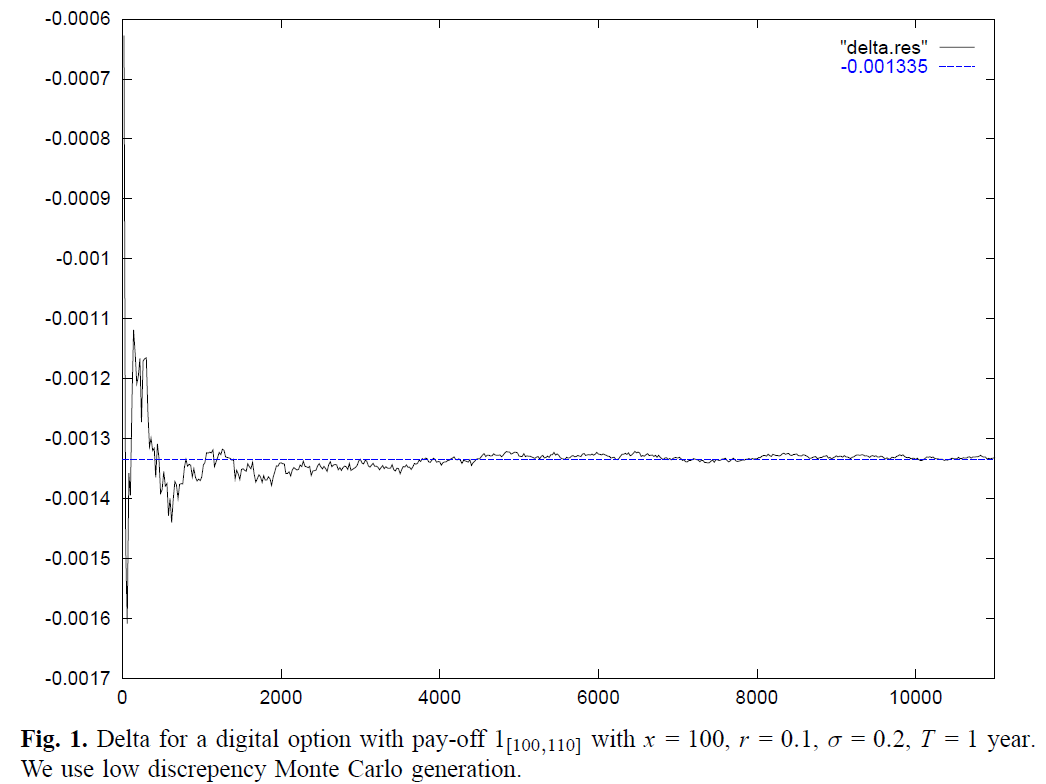
\includegraphics[scale=0.3]{fig1_fournie_99_malliavin_mc.png}\\
  %\caption{}\label{}
\end{figure}
\end{frame}

\begin{frame}
  \begin{figure}
  \centering
  % Requires \usepackage{graphicx}
  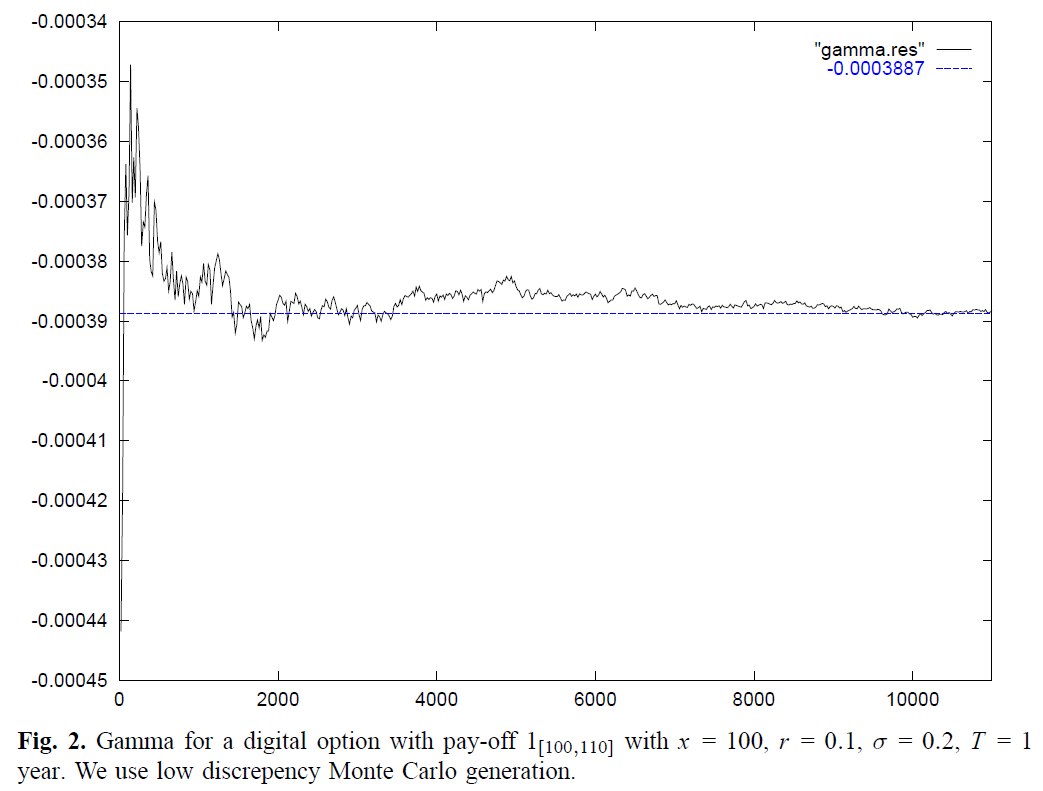
\includegraphics[scale=0.3]{fig2_fournie_99_malliavin_mc.png}\\
  %\caption{}\label{}
\end{figure}
\end{frame}

\begin{frame}
  \begin{figure}
  \centering
  % Requires \usepackage{graphicx}
  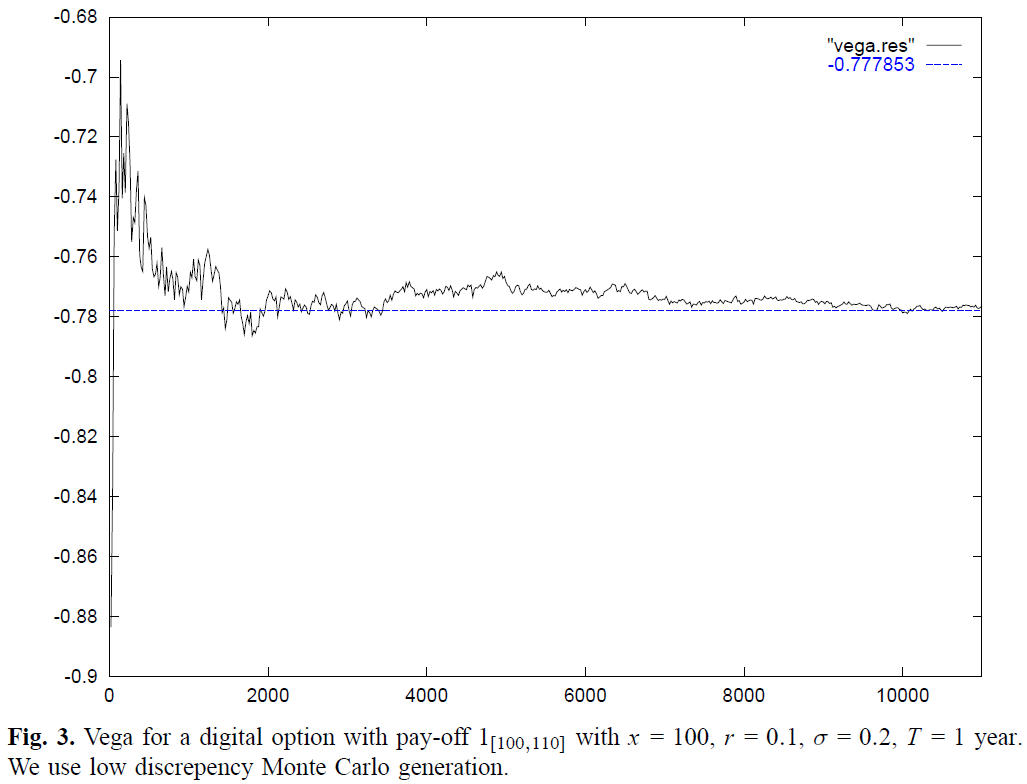
\includegraphics[scale=0.3]{fig3_fournie_99_malliavin_mc.png}\\
  %\caption{}\label{}
\end{figure}
\end{frame}

\begin{frame}
  \begin{figure}
  \centering
  % Requires \usepackage{graphicx}
  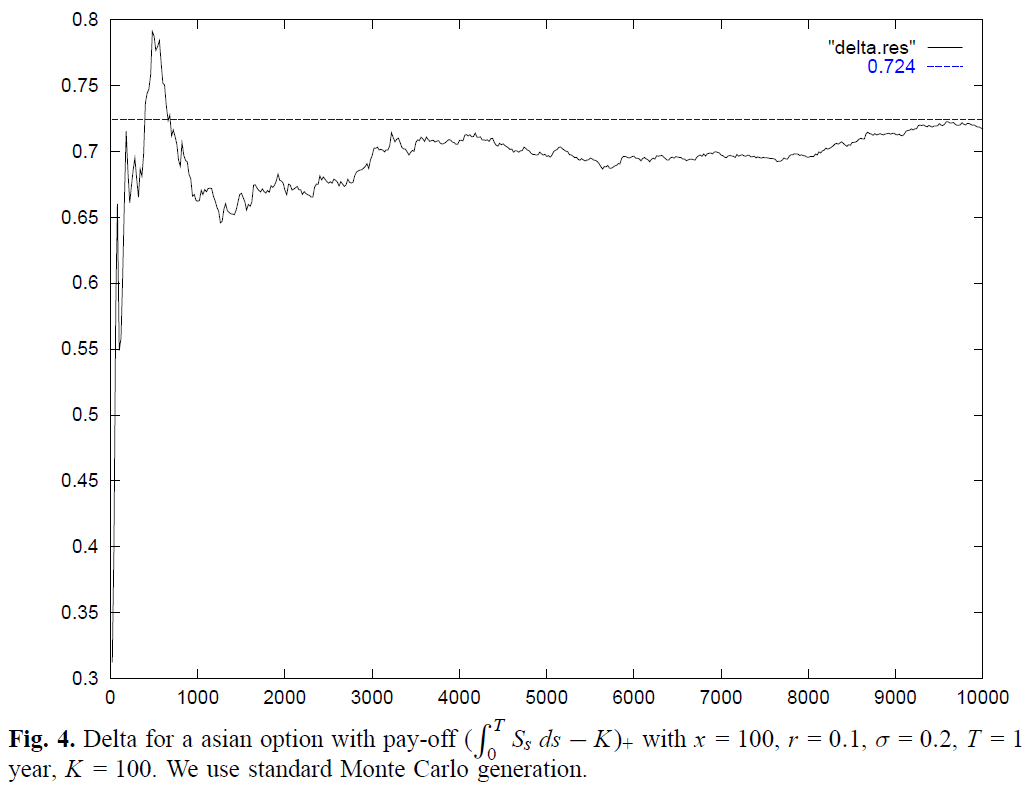
\includegraphics[scale=0.3]{fig4_fournie_99_malliavin_mc.png}\\
  %\caption{}\label{}
\end{figure}
\end{frame}

\begin{frame}
  \begin{figure}
  \centering
  % Requires \usepackage{graphicx}
  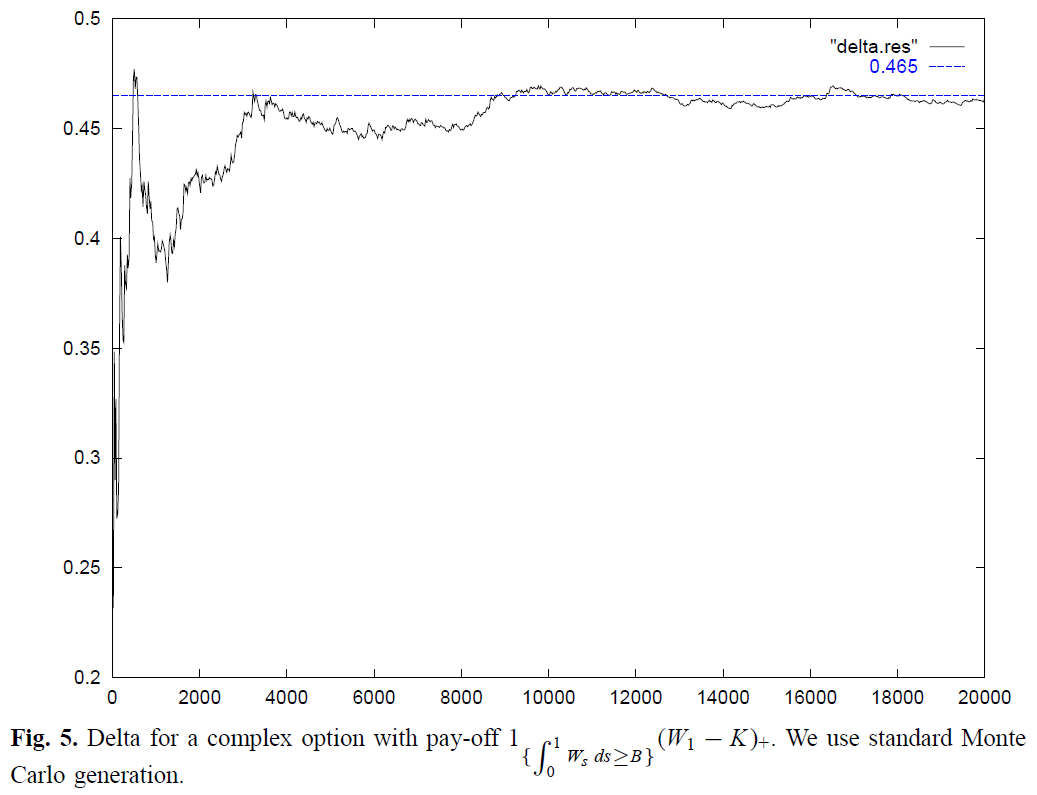
\includegraphics[scale=0.3]{fig5_fournie_99_malliavin_mc.png}\\
  %\caption{}\label{}
\end{figure}
\end{frame}

\begin{frame}
  \begin{figure}
  \centering
  % Requires \usepackage{graphicx}
  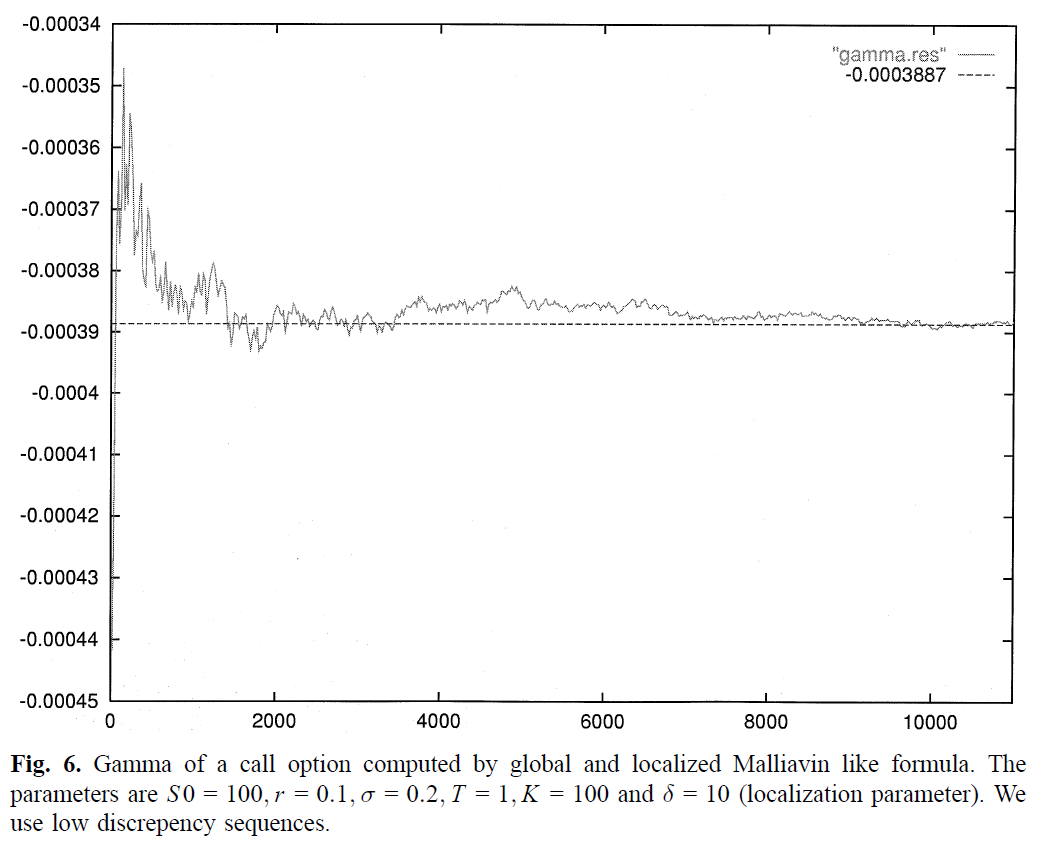
\includegraphics[scale=0.3]{fig6_fournie_99_malliavin_mc.png}\\
  %\caption{}\label{}
\end{figure}
\end{frame}

\begin{frame}
  \begin{figure}
  \centering
  % Requires \usepackage{graphicx}
  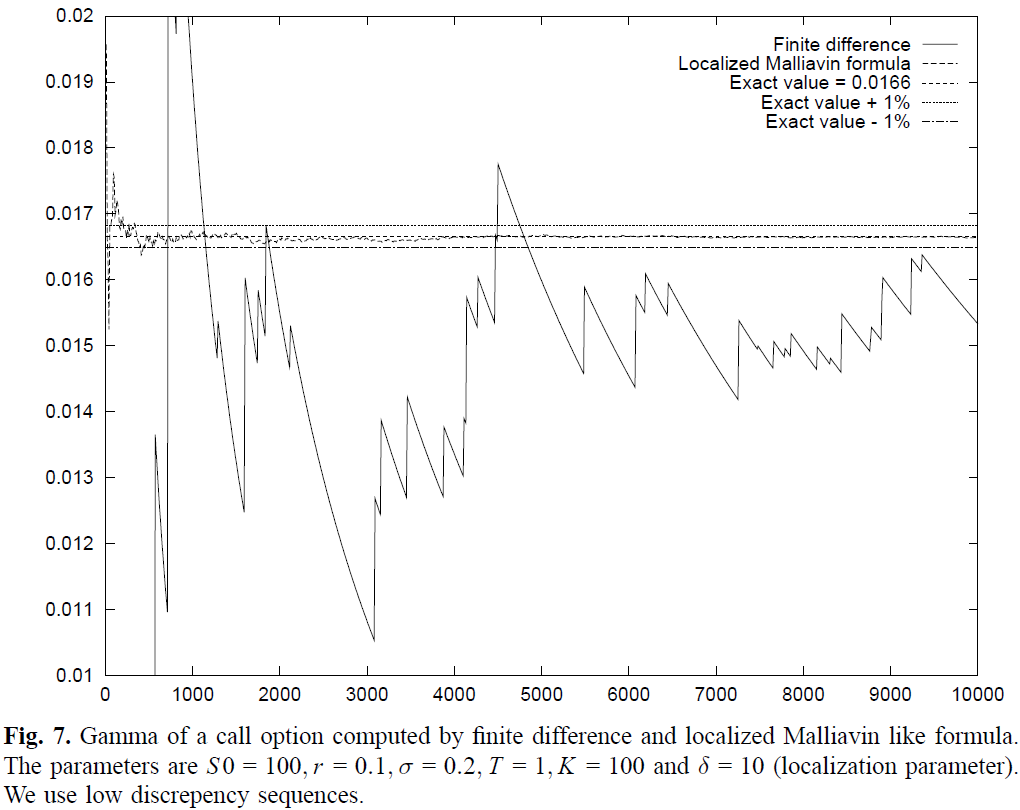
\includegraphics[scale=0.3]{fig7_fournie_99_malliavin_mc.png}\\
  %\caption{}\label{}
\end{figure}
\end{frame}

\begin{frame}
  \begin{figure}
  \centering
  % Requires \usepackage{graphicx}
  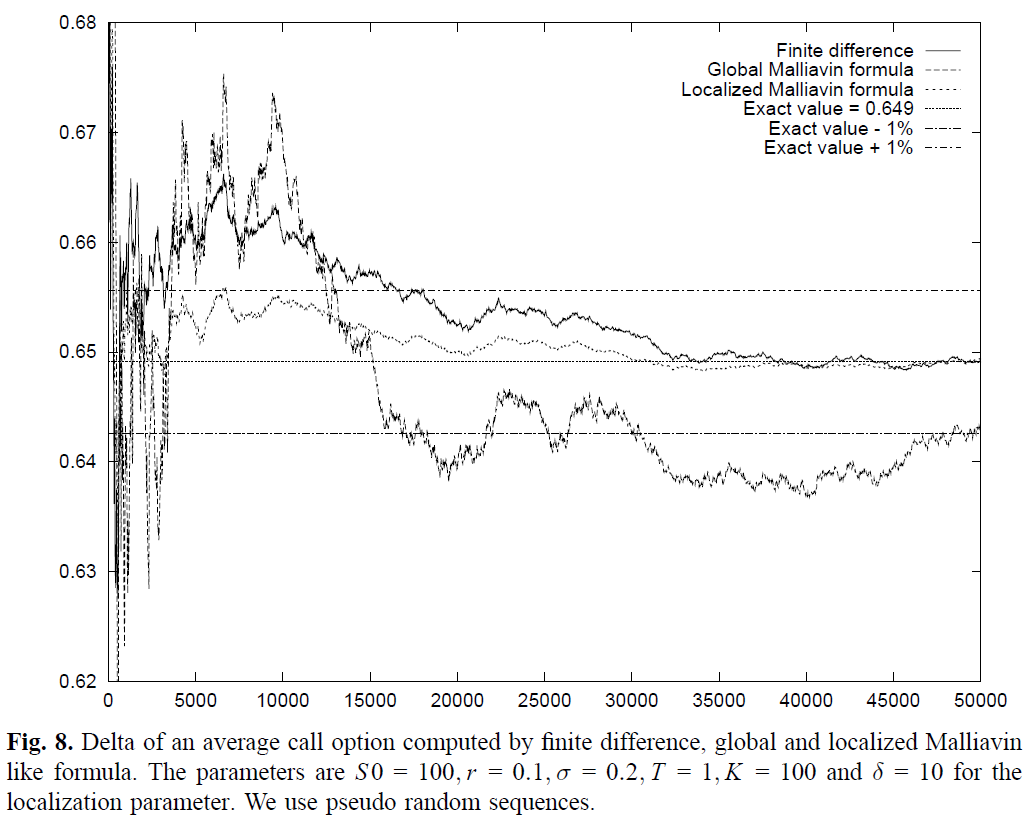
\includegraphics[scale=0.3]{fig8_fournie_99_malliavin_mc.png}\\
  %\caption{}\label{}
\end{figure}
\end{frame}

%%%%%%%%%%%%%%%%%%%%%%%%%%%%%%%%%%%%%%%%%%%%%%%%%%%%%%%%%%%%%%

\section{Summary}

%%%%%%%%%%%%%%%%%%%%%%%%%%%%%%%%%%%%%%%%%%%%%%%%%%%%%%%%%%%%%%

\section{Reference}

\begin{frame}{Reference}
  \begin{figure}
  \centering
  % Requires \usepackage{graphicx}
  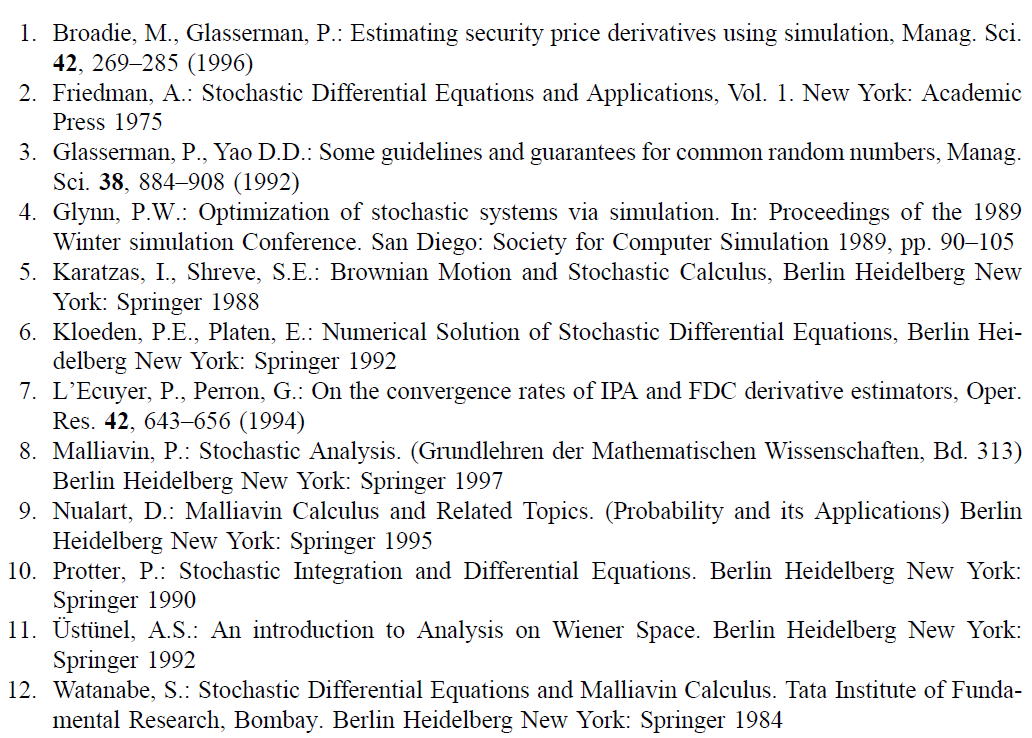
\includegraphics[scale=0.3]{reference.png}\\
  %\caption{}\label{}
\end{figure}
\end{frame}


\end{document}